\listfiles
\documentclass[review]{elsarticle}

\usepackage{lineno,hyperref}
\usepackage{multirow}
\usepackage{amsmath}
\usepackage{bbm}
\usepackage[utf8]{inputenc}
\usepackage{xurl}
% \modulolinenumbers[5]

% \usepackage{titlesec}

\setcounter{secnumdepth}{4}
\setcounter{tocdepth}{4}

% \titleformat{\paragraph}
% {\normalfont\normalsize\itshape}{\theparagraph}{0.5em}{}
% \titlespacing*{\paragraph}
% {0pt}{3.25ex plus 1ex minus .2ex}{1.5ex plus .2ex}

\journal{Renewable \& Sustainable Energy Reviews}

%%%%%%%%%%%%%%%%%%%%%%%
%% Elsevier bibliography styles
%%%%%%%%%%%%%%%%%%%%%%%
%% To change the style, put a % in front of the second line of the current style and
%% remove the % from the second line of the style you would like to use.
%%%%%%%%%%%%%%%%%%%%%%%

% Numbered
% \bibliographystyle{model1-num-names}

%% Numbered without titles
% \bibliographystyle{model1a-num-names}

%% Harvard
% \bibliographystyle{model2-names}\biboptions{authoryear}

%% Vancouver numbered
% \usepackage{numcompress}\bibliographystyle{model3-num-names}

%% Vancouver name/year
% \usepackage{numcompress}\bibliographystyle{model4-names}\biboptions{numbers}

%% APA style
% \bibliographystyle{model5-names}\biboptions{authoryear}

%% AMA style
% \usepackage{numcompress}\bibliographystyle{model6-num-names}

%% `Elsevier LaTeX' style, distributed in TeX Live 2019
\bibliographystyle{elsarticle-num}
% \usepackage{numcompress}\bibliographystyle{elsarticle-num-names}
% \bibliographystyle{elsarticle-harv}\biboptions{authoryear}

\biboptions{sort&compress}
%%%%%%%%%%%%%%%%%%%%%%%

\begin{document}
\begin{frontmatter}

\title{Calibrating building energy simulation models: A review of methods, inputs and outputs}


%% Group authors per affiliation:
\author[add1]{Adrian Chong\corref{mycorrespondingauthor}}
\cortext[mycorrespondingauthor]{Corresponding authors}
\ead{adrian.chong@nus.edu.sg}
\author[add1]{Yaonan Gu}
\author[add2]{Hongyuan Jia}

\address[add1]{Department of Building, School of Design and Environment, National University of Singapore, 4 Architecture Drive, Singapore 117566, Singapore}
\address[add2]{SinBerBEST Program, Berkeley Education Alliance for Research in Singapore, Singapore, 138602, Singapore}


\begin{abstract}
Building energy simulation (BES) plays a significant role in buildings with applications such as Architectural design, retrofit analysis, and optimizing building operation and controls. There is a recognized need for model calibration to improve the simulations' credibility, especially with building data becoming increasingly available and the promises that a digital twin brings. However, there is currently no consensus on the procedures concerning BES calibration. This study aims to provide the foundation for future research through a detailed systematic review of the vital aspects of BES calibration. Specifically, we conducted a meta-analysis and categorization of the simulation inputs and outputs, data type and resolution, key calibration methods, and calibration performance evaluation. This study also identified reproducible simulations as a critical issue and proposes an incremental approach to encourage future research's reproducibility. 

\section*{Highlights}
\begin{itemize}
    \item The first systematic review of model calibration in building simulation.
    \item Meta-analysis to understand better the inputs and outputs used for calibration. 
    \item Optimization and Bayesian calibration are the most common automated approach.
    \item Literature does not distinguish between model credibility and predictive accuracy.
    \item Reproducibility is a critical issue and needs to be encouraged in future research.
\end{itemize}

\end{abstract}
%TC:ignore
\begin{keyword}
Building performance simulation \sep Building simulation \sep calibration \sep reproducibility \sep Optimization \sep Uncertainty
\end{keyword}
%TC:endignore

\end{frontmatter}

%TC:ignore
Word Count: 8146
%TC:endignore

% \linenumbers
\section{Introduction}

\subsection{Calibration in building energy simulation}
Building energy simulation (BES) can generally be defined as a physics-based mathematical model that allows the detailed calculation of a building's energy performance and occupant thermal comfort under the influence of various inputs such as weather, building geometry, internal loads, HVAC systems, operational schedules, and simulation specific parameters. Original intended for use during the design phase, BES is increasingly being used throughout a building's lifecycle \cite{hensen2019building}. However, there are increasing concerns about the model's credibility within the building industry as significant discrepancies between simulated and measured energy use becomes more apparent with the rapid deployment of smart energy meters and the internet of things (IoT) \cite{de2014gap}. For instance, Turner and Frankel \cite{turner2008energy} analyzed 121 LEED buildings and found that measured energy use can be between 0.5 to 2.75 times the predicted energy use. Mantesi et al. \cite{mantesi2018modelling} showed that default settings and methods of modeling thermal mass can result in up to 26\% divergence in the simulation predictions. 

Previous studies \cite{menezes2012predicted, de2002analysis} observed that the main causes of discrepancies between predicted and actual energy performance stem from: (a) specification uncertainty arising from assumptions due to a lack of information; (b) model inadequacy arising from simplifications and abstractions of actual physical building systems; (c) operational uncertainty arising from a lack of feedback regarding actual use and operation of buildings; and (d) scenario uncertainty arising from specifying model conditions that include among other things weather conditions and building occupancy. Consequently, model calibration is often undertaken to match simulation predictions to actual observations better and increase the model's credibility for making predictions. Although calibration is not essential for BES research, it is becoming increasingly important for establishing model credibility. The International Energy Agency's Energy in Buildings and Communities (IEA-EBC) Annex 53 also reported the significance of the development and application of model calibration and uncertainty analysis for BES \cite{yoshino2017iea}. 

The typical reason for BES calibration is to more confidently predict using simulation. Although predictions may be wrong, they can still be useful. Trucano et al. \cite{trucano2006calibration} list examples of such predictions that are also relevant for BES, and they include: 
\begin{itemize}
    \item Simulate an experiment without knowledge of its results or prior to its execution. Examples include retrofit analysis such as comparing the cost-effectiveness of different energy conservation measures (ECMs) and building performance optimization.
    \item Make scientific pronouncements about phenomena that cannot currently be studied experimentally. Examples include observations of changes in building energy performance considering different climate change scenarios or a scenario where occupancy and building usage can become sporadic in the event of a pandemic.
    \item Use computation to extrapolate existing understanding into experimentally unexplored regimes, such as using BES to create a baseline for quantifying energy savings for buildings with multiple interactive ECMs.
\end{itemize}

\subsection{Calibration, validation, and verification}

Calibration, validation, and verification have been used conversely in the existing literature to indicate consistency between model predictions and actual observations, which can be misleading since they are not synonymous. The semantics of the words calibration, validation, and verification have been subject to philosophical debates because of the paradoxical view that models are a representation of reality and thus by definition not true \cite{oreskes1994verification}. As such, there have been arguments that simulation models can never be validated but can only be improved through invalidation \cite{konikow1992ground}. Nevertheless, BES models are typically built for practical purposes such as for architectural design, HVAC design and operation, retrofit analysis, building operational optimization, urban-scale energy efficiency analysis, etc. Therefore, from a computational simulation and engineering perspective, the idea of validation is not to establish the truth of a scientific theory but to evaluate and quantify if the model is acceptable for its intended purpose. 

Within this context, BES calibration, validation, and verification can be formally defined following the guide by the American Institute of Aeronautics and Astronautics (AIAA) \cite{american1998aiaa}, which is also compatible with the US Department of Energy’s Advanced Simulation and Computing's (ASC) definitions \cite{trucano2006calibration}:

\begin{description}
    \item[Calibration]: The process of adjusting numerical or physical modeling parameters in the computational model for the purpose of improving agreement with experimental data.
    \item[Validation]: The process of determining the degree to which a model is an accurate representation of the real world from the perspective of the intended uses of the model. 
    \item[Verification]: The process of determining that a model implementation accurately represents the developer's conceptual description of the model and the solution to the model.
\end{description}

\subsection{Related work}
Over the past two decades, three literature review articles \cite{reddy2006literature, coakley2014review, fabrizio2015methodologies} have been published regarding BES calibration. In 2005 as part of an ASHRAE initiated research project (RP-1051), Reddy \cite{reddy2006literature} classified calibration methodologies from existing literature into four classes: (1) calibration based on manual, iterative, and pragmatic intervention; (2) calibration based on a suite of informative graphical comparative displays; (3) calibration based on specific tests and analytical procedures; and (4) analytical/mathematical methods of calibration. In 2014, Coakley, Raftery, and Keane \cite{coakley2014review} extended these classifications to include advancements in optimization techniques, Bayesian calibration, and alternative modeling techniques such as meta-modeling. Additionally, a broader definition of calibration approaches as either manual or automated was proposed. In the following year, Fabrizio and Monetti \cite{fabrizio2015methodologies} built upon the study by Coakley, Raftery, and Keane \cite{coakley2014review} by discussing in further detail the issues affecting BES calibration. 

\subsection{Aim and objectives}
Although there have been numerous BES calibration studies over the past decade, most studies focused on applying a specific calibration methodology to specific case study buildings. Combined with the lack of open code and data, BES calibration remains challenging to replicate. Additionally, as described in the preceding paragraph, existing review articles focus on providing an overview of current calibration methodologies. However, proper specification of model inputs and outputs is equally important. To date, there has been little quantitative analysis about model inputs and outputs, calibration methods, and the criteria for evaluating calibration performance. The determination of all these details is highly subjective, often requiring a high level of expertise, experience, and domain knowledge. Despite its importance, there is little guidance on best practices to facilitate reproducible research regarding BES calibration. 

With the aim of enhancing reproducibility and enabling others to build upon published work more easily, the objectives of this review article are to:
\begin{itemize}
    \item Synthesize relevant BES literature and the relationship between various model inputs and outputs.
    \item Perform a detailed meta-analysis of the calibration methods and measures of calibration performance currently utilized in the existing literature. 
    \item Provide recommendations to facilitate reproducibility in BES.
\end{itemize}

We believe that meeting these objectives will provide a solid foundation and platform for future research to advance the current state of BES calibration. This is also the first systematic review on the subject.

\section{Method} \label{sec:method}

A systematic review was adopted to provide a comprehensive and unbiased summary of evidence on model inputs/outputs, calibration performance metrics, and calibration methods.

\subsection{Search and eligibility criteria}

Table \ref{tab:search_criteria} presents the search strategy used to identify relevant publications from the Scopus database. The keywords ``model calibration'' and ``building energy simulation'' were used to identify an initial list of publications. To capture as many relevant publications as possible, synonyms that are interchangeable with ``model calibration'' and ``building energy simulation'' in the BES literature were included in the search string. 

The initial search returned 2,762 publications. Limiting the search to English journal articles published between 2015 and 2020 resulted in 781 publications. We limit the review to the immediate past six years to reflect recent trends and state-of-the-art in BES. Additionally, the most recent review paper for BES calibration was in the year 2014 \cite{coakley2014review} and 2015 \cite{fabrizio2015methodologies}. 

Further refinements to the search criteria were made by including relevant subject areas (Engineering, Environmental Science, and Energy) and explicitly excluding irrelevant subject areas (Material science, Social Sciences, and Chemical engineering). These criteria excluded 338 studies and left 443 for the review. The titles and abstracts of the 443 studies were subsequently screened to identify relevant publications and their corresponding source journal, yielding 186 publications. 

\begin{table*}[h!]
\caption{Search criteria for systematic literature review} 
\label{tab:search_criteria}
\centering
\resizebox{\textwidth}{!}{\begin{tabular}{|p{0.3\linewidth} | p{0.7\linewidth}| }
  \hline
  Criteria & Description \\
  \hline
  \multirow{2}{*}{Keywords} &  [``calibration'' OR ``model calibration''] AND \\
  & [``building performance simulation''  OR ``building energy model'' OR ``building energy modeling'' OR ``building energy simulation'' OR``building simulation'' OR ``energy simulation'' OR ``whole building energy model''] \\
  \hline
  Database & Scopus \\
  \hline
  Search date & 16 January 2021 \\
  \hline
  \multirow{6}{*}{Limit to}& Year: 2015-2020 \\
  & Language: English \\
  & Document type: Article \\
  & Source type: Journal \\
  & Subject areas: Engineering, Environmental Science, Energy \\
  & Journals: Energy and Buildings, Applied Energy, Automation in Construction, Building and Environment, Solar Energy, Applied thermal energy, Journal of Building Performance Simulation, Journal of Building Engineering, Building Simulation, HVAC and R Research\\
  \hline
  Exclude & Subject areas: Material science, Social Sciences, Chemical engineering \\
  \hline
  \multicolumn{2}{|c|}{Total number of publications returned: 186} \\
  \hline
\end{tabular}}
\end{table*}

\subsection{Study selection}

The full papers of the 186 publications were subsequently screened for relevance to this review based on the following criteria: (1) the study involved the use of building energy simulation; (2) the study contains the application of calibration methods or techniques; and (3) the study is not vague on the proposed calibration approach and is not ambiguous on the model input(s) and output(s). Of the 186 studies, 107 were selected for the review.

\section{Categorization}

\subsection{Simulation engine}

Table \ref{tab:sim_engine} displays the breakdown of the papers reviewed according to the simulation engine used. A majority of the papers reviewed (60\%) used EnergyPlus for a variety of reasons. EnergyPlus is an open-source whole-building energy simulation engine that has been and continues to be supported by the U.S. Department of Energy (DOE) \cite{doe_energyplus}. Moreover, EnergyPlus supports many application software \cite{ibpsa_best}. Examples from this review include DesignBuilder \cite{designbuilder}, OpenStudio \cite{guglielmetti2011openstudio}, jEPlus \cite{jeplus}, and GenOpt \cite{wetter2001genopt}. 

15\% and 7\% of the papers reviewed use TRNSYS and DOE-2 respectively. TRNSYS \cite{klein2017trnsys} is a transient systems simulation program that is designed to provide flexibility in conducting energy simulations through a modular structure and extensive add-on component libraries. Additionally, TRNSYS is also supported by application softwares jEPlus \cite{jeplus} and GenOpt \cite{wetter2001genopt}. DOE-2 \cite{doe2} is a building energy simulation program that performs hourly simulation given descriptions of the building layout, constructions, operating schedules, HVAC systems, and utility rates. 

What stands out in Table \ref{tab:sim_engine} is that Resistance-Capacitance (RC) networks (also known as lumped parameter models) were used in 10\% of the studies reviewed. Unlike the other three commonly used white box simulation engines (EnergyPlus, TRNSYS, and DOE-2), an RC network is a gray-box model \cite{li2014review}. White box models use dynamic physics-based equations to model a building's component, sub-system, and system. In contrast, gray box models are hybrid models that combine simplified physical representations of the building with operation data that are used to identify the model's coefficients. The benefits of an RC network lies in having physical descriptions of the building while being computationally more efficient than white-box models. Further easing implementation, the development of RC models may also follow the well-established international standard ISO 13790:2008 \cite{iso13790energy} that was subsequently revised by ISO 52016-1:2017 \cite{iso52016energy}.

\begin{table*}[h!]
\caption{Simulation engines used in the reviewed calibration applications ($N=107$).} 
\label{tab:sim_engine}
\centering
\resizebox{\textwidth}{!}{\begin{tabular}{l c c}
  \hline
  Simulation Engine & Type & Percentage of Papers Reviewed \\
  \hline
  EnergyPlus & \multirow{3}{*}{white-box} & 60\%\\ 
  TRNSYS & & 15\% \\
  \hline
  Resistance-Capacitance (RC) & Gray-box & 10\% \\
  \hline
  Others & NA & 8\% \\
  \hline
\end{tabular}}
\end{table*}

\subsection{Spatial and temporal scales}

Fig. \ref{fig:spatial_temporal} compares the temporal resolution of the output responses used for the calibration across different spatial scales of the BES models. It can be seen from the data in Fig. \ref{fig:spatial_temporal} that the temporal resolution of the data used to calibrate the models decreases with increasing simulation scales. A closer inspection of the figure shows that (a) models of building components and sub-systems are often calibrated using sub-hourly or hourly data; (b) whole building energy models are usually calibrated using hourly or monthly data; (c) about two-thirds of the urban-scale building energy models (UBEM) are calibrated with monthly or annual data while the remaining applications used hourly data, (d) the coarsest resolution of data used for the calibration of component/system, building, and urban scale models are hourly, monthly and annual respectively. 

\begin{figure}[!h]
\centering
\includegraphics[width=0.7\textwidth]{figures/spatial_temporal_stacked.pdf}
\caption{Percentage breakdown of the temporal resolution of the measured output used to guide the calibration of the energy models across different spatial scales.}
\label{fig:spatial_temporal}
\end{figure}

Fig. \ref{fig:map_climate} shows the geographic distribution of the case study buildings extracted from the papers reviewed across various simulation scales (top map plot) and within each k\"{o}ppen climate zones (bottom bar-plot). Looking at the map in Fig. \ref{fig:map_climate}, it is apparent that a majority of case study applications are located in the U.S. or Europe, with several in China and South Korea. These applications are situated between latitude 30$^{\circ}$N and 65$^{\circ}$N. Consequently, 96\% of the studies belong to an arid (dry), temperate (mild mid-latitude), or continental (cold mid-latitude) climate group. Only 4\% of the applications were in the equatorial region characterized by a warm and humid climate all year round. 

An inspection of the data in Fig. \ref{fig:map_climate} reveals that over three-quarters of the case studies are at the building scale (77\%). 15\% at the urban-scale and the remaining 8\%\footnote{8\% does not include whole building calibration studies that employ multi-stage or sequential calibration approaches that utilize the calibration of a single building component or system as part of the process.} for the calibration of a single building component or system. A further observation that emerged from the data was that urban-scale case studies are located only in the U.S. (54\%), Europe (34\%), and the Middle East (12\%). None of the urban-scale studies were located in the tropics.

\begin{figure}[!h]
\centering
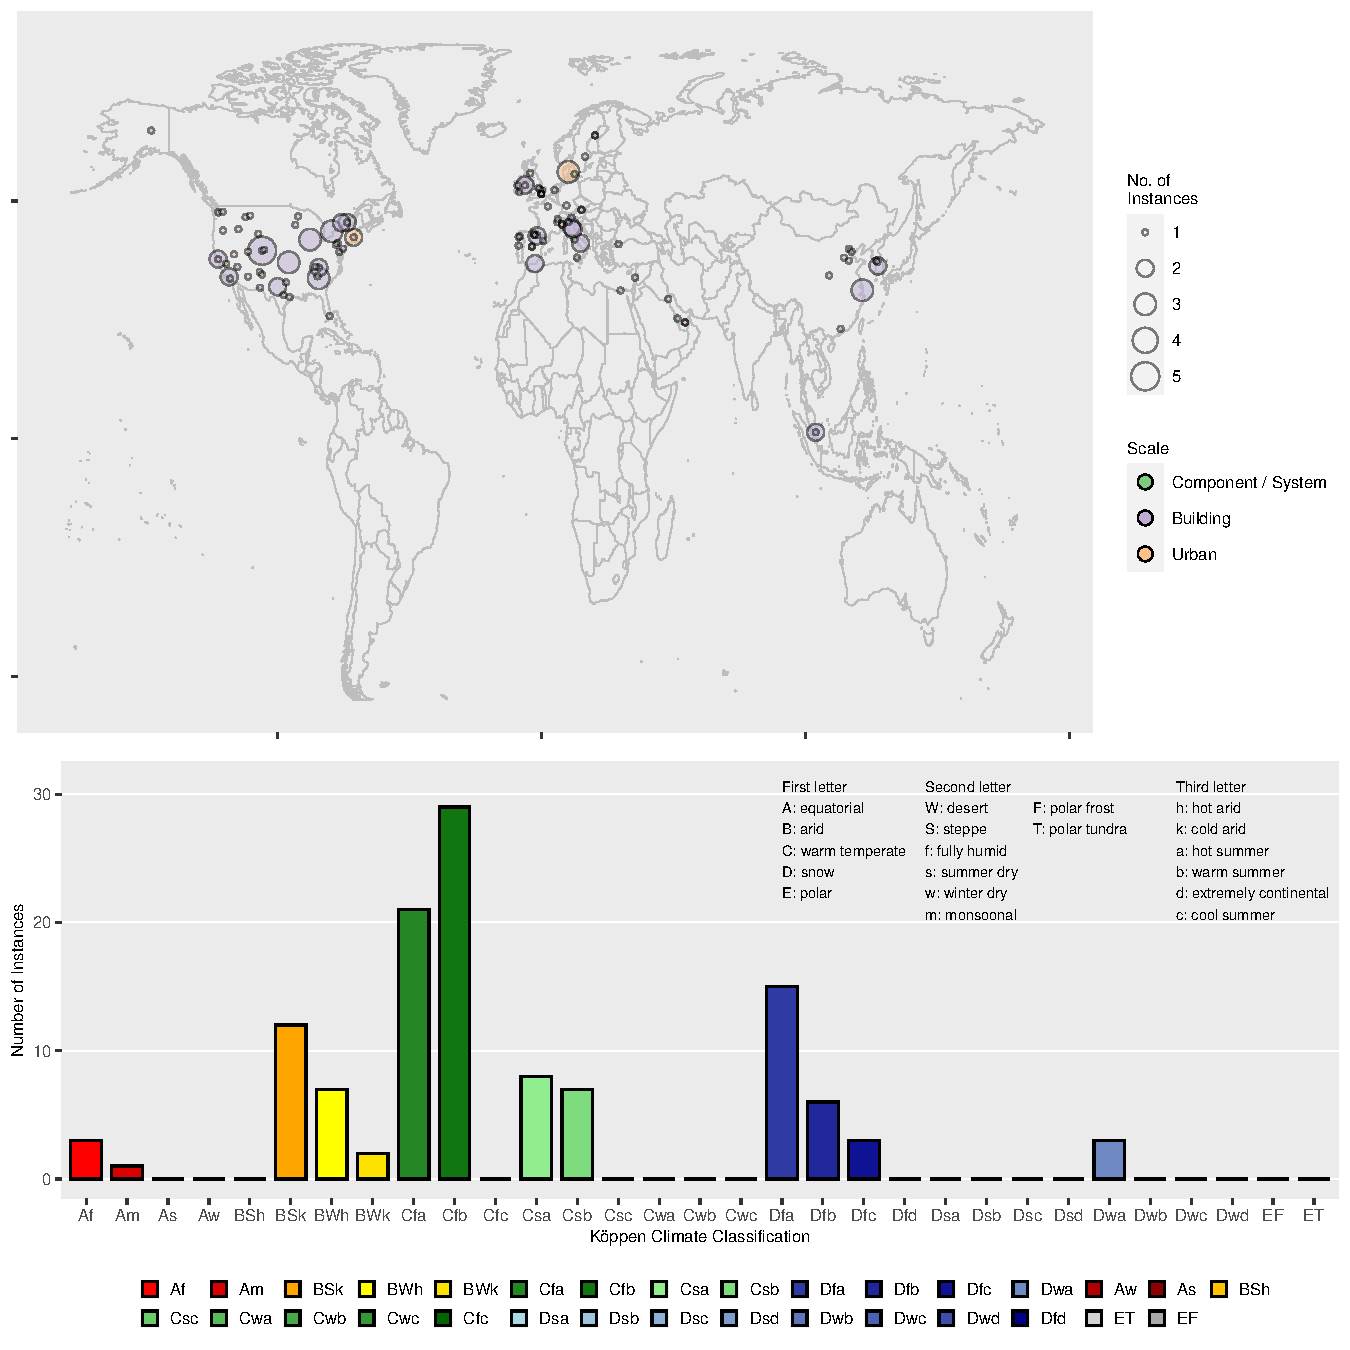
\includegraphics[width=1.1\textwidth]{figures/map_climate.pdf}
\caption{Geographic distribution of case study buildings and the corresponding scale of the simulation (component/system, building, or urban) (top plot) and the distribution of the case study buildings based on the k\"{o}ppen climate zones (bottom plot.}
\label{fig:map_climate}
\end{figure}


\section{Modeling and data requirements}

\subsection{Input, output, and parameter mapping}

As illustrated in Fig. \ref{fig:morphism}, BES models are representations of aspects of reality that are manipulated and experimented with using a variety of simulations \cite{augenbroe2019role, aumann2007methodology}. Therefore, the goal is to have models be adequately representative of actual building performance over a sufficiently wide range of inputs that encompasses the simulation aim and thus application. Since BES models are complex computer models with an enormous number of inputs and outputs, a comparison of the input and output mapping is carried out through a meta-analysis of the existing literature. We define three categories of inputs/outputs with reference to Fig. \ref{fig:morphism}:
\begin{description}
    \item[Observed input(s)]: Model input parameters whose value could be determined from available evidence or data. These parameters can be directly observed (e.g., outdoor dry-bulb temperature and relative humidity from local weather stations) or derived/estimated (e.g., infiltration rate derived from blower door tests).
    \item[Calibration parameter(s)]: Model input parameters that are tuned to match simulated output(s) to observed output(s).
    \item[Observed output(s)]: Observable model output(s) of interest that is used to guide the tuning of the calibration parameter(s). 
\end{description}

\begin{figure}[!h]
\centering
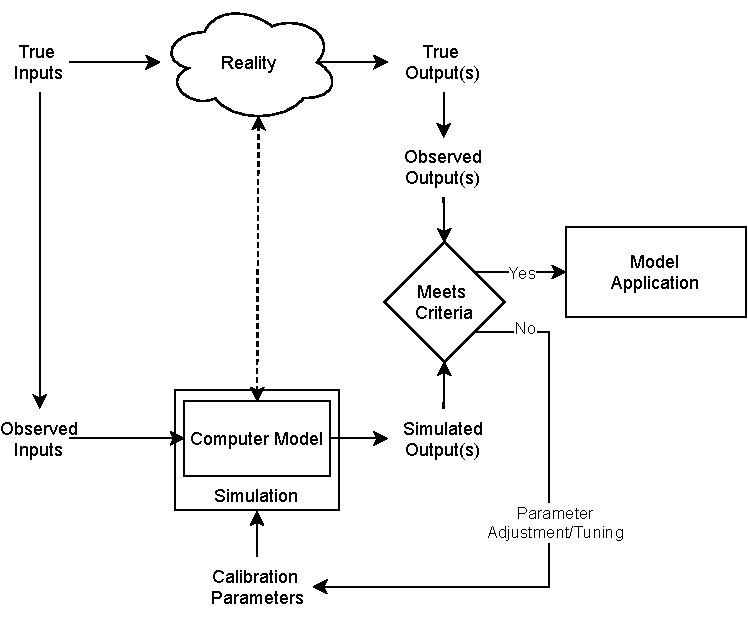
\includegraphics[width=0.8\textwidth]{figures/morphism.pdf}
\caption{Schematic illustrating the calibration process given that the simulation is a representation of reality.}
\label{fig:morphism}
\end{figure}

\subsubsection{Most common observed inputs and outputs}

It is apparent from Fig \ref{fig:target} that building level data that includes electricity and gas/steam energy, heating and cooling load/energy, and total load/energy are most frequently used for the calibration of energy models. A possible explanation is an increasing availability and accessibility to building level measurements such as utility meters. This has also led to model calibration efforts at the urban scale using electricity and/or gas consumption data \cite{santos2018evaluating, sokol2017validation, nagpal2019framework, chen2020automatic, krayem2019urban}. Measured zone indoor air dry-bulb temperature is the second most frequently used output to guide the calibration process. Specifically, the adjustment of parameters using indoor air temperature is often carried out during free-floating periods when the indoor temperatures are allowed to float without any HVAC system intervening. Consequently, outdoor air temperature is also frequently monitored concurrently to provide the boundary conditions of the simulation \cite{martinez2019energy, figueiredo2018comparison, lee2018improvements, andrade-cabrera2017ensemble, mylona2017frozen, elharidi2017energy, tokarik2016life, ramosruiz2016genetic, roberti2015calibrating, cipriano2015evaluation, derosa2019iterative, zuhaib2019application, lundstrom2019bayesian, aparicio-fernandez2019energy, cornaro2017energy, ferrara2020optimizing}.

Fig. \ref{fig:input} provides an overview of the most commonly used observed inputs. What stands out from Fig. \ref{fig:input} is the obvious use of local weather data (dry bulb temperature, solar radiation, relative humidity, wind speed and direction) as observed inputs to the model. If local site measurements are not available, an annual meteorological year (AMY) weather file from the nearest weather station is used. These observations indicate the importance of using actual weather data for the calibration since the weather file forms the energy simulation's boundary conditions. The weather file's importance was also demonstrated in previous research that showed that the annual building energy consumption and the monthly building loads could vary by $\pm$7\% and $\pm$40\%, respectively, based on the provided weather data \cite{bhandari2012evaluation}.

\begin{figure}[!h]
\centering
\includegraphics[width=\textwidth]{figures/target_byLevel.pdf}
\caption{Most common observed outputs used for calibrating building energy simulation models. The color indicates the spatial resolution of the observation.}
\label{fig:target}
\end{figure}

\begin{figure}[!h]
\centering
\includegraphics[width=\textwidth]{figures/input_byLevel.pdf}
\caption{Most common observed inputs used for calibrating building energy simulation models. The color indicates the class of the model parameter.}
\label{fig:input}
\end{figure}

Interestingly, several studies used measured indoor environmental conditions as inputs to the model to obtain a model that is better calibrated at the zone level. For instance, Mihai and Zmeureanu \cite{mihai2017bottom} showed that using measured indoor air temperatures in place of those from the technical specification led to more accurate predictions of zone airflow rates. Yin, Kiliccote, and Piette \cite{yin2016linking} used air temperature and airflow measurements to derive the zone thermostat setpoint and the VAV box minimum/maximum airflow respectively. Infiltration rate is sometimes derived from measurements because it is highly uncertain and can have significant influence on a building's energy use \cite{persily2010modeled}. In this review, infiltration rates are typically derived from airtightness values that are obtained using the blower door test \cite{kim2018model, bandera2017towards, vesterberg2016calibration, ramosruiz2016genetic, roberti2015calibrating, zuhaib2019application, fernandez2020novel, escandon2017assessment}.

\subsubsection{Observed outputs and calibration parameters mapping} \label{sec:output_param}

Fig. \ref{fig:param} lists the model parameters that were most commonly adjusted to match simulation output to the observations. Data from Fig. \ref{fig:param} was used to generate Fig. \ref{fig:target_param}, which shows the magnitude of the relationship between the most commonly used calibration parameters and their corresponding observed outputs. The mapping reveals that parameters concerning the building envelope (material properties and infiltration rate), internal gains (occupant, lighting, and equipment power density), and zone cooling and heating setpoints are often adjusted when calibrating the energy model to building electricity energy consumption. Closer inspection of the first column of Fig. \ref{fig:target_param} shows that HVAC component efficiency and zone outdoor air levels were also calibrated in a considerable number of papers. Not surprisingly, hot water usage was also adjusted in several studies that were calibrating models of residential typologies \cite{nagpal2019methodology, sokol2017validation, robertson2015reduced, manfren2020parametric}. About six to seven articles calibrated the internal loads' schedule \cite{nagpal2019methodology, kim2017building, sun2016pattern, nagpal2019framework, asadi2019building, chen2020automatic, krayem2019urban}. Previous studies have demonstrated the importance of schedule adjustment in model calibration \cite{kim2017building, chong2021occupancy}. However, schedules are difficult to adjust due to the potentially large number of parameters. Therefore, schedule adjustment typically involves simplification, such as selecting from a list of predefined discrete schedules that best fit the measured data \cite{nagpal2019methodology, nagpal2019framework, krayem2019urban, chen2020automatic}. 

\begin{figure}[!h]
\centering
\includegraphics[width=\textwidth]{figures/param_byLevel.pdf}
\caption{Most common calibration parameters used for calibrating building energy simulation models. The color indicates the class of the model parameter.}
\label{fig:param}
\end{figure}

\begin{figure}[!h]
\centering
\includegraphics[width=\textwidth]{figures/target_parameter_point.pdf}
\caption{The magnitude of the relationship between the calibration parameters and their corresponding observed outputs for calibrating building energy simulation models.}
\label{fig:target_param}
\end{figure}

Fig. \ref{fig:target_param} reveals several other interesting observations. First, the same calibration parameters were used when calibrating against both building electricity and gas/steam energy consumption. Second, the parameters calibrated when matching simulation predictions to total building load/energy are somewhat similar, except that equipment and lighting schedules are less likely to be adjusted. 

Turning to zone dry-bulb temperature as the observed output, parameters concerning envelope material properties are the most commonly adjusted, followed by infiltration rate. A similar observation can be made when the model is calibrated to the building's heating or cooling load/energy. Material properties and infiltration rate are selected because indoor temperature measurements are often used to investigate the relative changes in the building envelope performance with varying boundary conditions \cite{lee2018improvements, figueiredo2018comparison, cacabelos2017development, enriquez2017towards}. Additionally, studies have found parameters affiliated with infiltration rate and material properties to influence on indoor air temperature \cite{martinez2019energy, enriquez2017towards, roberti2015calibrating, cipriano2015evaluation, ferrara2020optimizing}. 

Finally and intuitively, Fig. \ref{fig:target_param} shows that HVAC component capacity and efficiency are typically adjusted when the observed output is the HVAC component's energy consumption. Likewise, EPD and equipment schedules are adjusted when the model is calibrated against equipment energy consumption. 

\subsection{Calibration performance evaluation}

\subsubsection{Current approaches} \label{sec:performance_current}

Table \ref{tab:metrics} ranks the metrics used to assess calibration performance based on the number of occurrences in the papers reviewed. A large proportion of the papers use CV(RMSE) or NMBE to determine if a BES model was calibrated. This result is not unexpected since BES models are often deemed ``calibrated'' if they meet the CV(RMSE) and NMBE limits (Table \ref{tab:error_limits}) specified by ASHRAE Guideline 14 \cite{ashrae2014guideline}, the International Performance Measurement and Verification Protocol (IPMVP) \cite{evo2012international}, or the Federal Energy Management Program (FEMP) \cite{femp2015guidelines}.

\begin{table*}[h!]
\caption{Metrics used for the evaluation of calibration performance. Each paper may employ more than a one metric when assessing calibration performance. Therefore, the cummulative sum for the column ``No. of Papers'' is greater than the total number of papers reviewed (N=107).} 
\label{tab:metrics}
\centering
\resizebox{\textwidth}{!}{\begin{tabular}{p{0.55\linewidth}  p{0.2\linewidth} P {0.25\linewidth}}
  \hline
  Metric & Acronym & No. of Papers \\
  \hline
  Coefficient of Variation of the Root Mean Square Error & $CV(RMSE)$ & 72 \\
  Normalized Mean Bias Error & $NMBE$ & 60 \\
  Root Mean Square Error & $RMSE$ & 18 \\
  Goodness of Fit & $GOF$ & 11 \\
  Coefficient of Determination & $R^2$ & 11 \\
  Annual Percentage Error & $APE$ & 8 \\
  Coefficient of Variation & $CV$ & 4 \\
  Mean Absolute Error & $MAE$ & 3 \\
  Mean Absolute Percentage Error & $MAPE$ & 3 \\
  Gelman-Rubin statistic & $\hat{R}$ & 3 \\
  Others$^\dagger$ & -- & 20  \\
  \hline
\end{tabular}}
\raggedright \tiny $\dagger$ Metrics with $\leq 2$ counts. 
\end{table*}

\begin{table*}[h!]
\caption{Error limits specified by various guidelines and protocols for a building energy simulation model to be deemed calibrated.} 
\label{tab:error_limits}
\centering
\resizebox{\textwidth}{!}{\begin{tabular}{c c c c c}
  \hline
  \multirow{2}{*}{Guideline / Protocol} & \multicolumn{2}{c}{Monthly Criteria (\%)} & \multicolumn{2}{c}{Hourly Criteria (\%)} \\
  \cline{2-5}
  & NMBE & CV(RMSE) & NMBE & CV(RMSE) \\
  \hline
  ASHRAE Guideline 14 \cite{ashrae2014guideline} & $\pm5$ & $15$ & $\pm10$ & $30$ \\
  IPMVP \cite{evo2012international} & -- & -- & $\pm5$ & 20 \\
  FEMP \cite{femp2015guidelines} & $\pm5$ & 15 & $\pm10$ & 30 \\
  \hline
\end{tabular}}
\end{table*}

CV(RMSE) (eq. \ref{eq:cvrmse}) provides an indication of how close the simulation predictions are to measured data while NMBE (eq. \ref{eq:nmbe}) serves as an indicator of overall bias in the simulation predictions. However, NMBE suffers from cancellation between positive and negative bias which can lead to misleading interpretations of predictive performance \cite{chakraborty2017performance}. This review also confirms the findings of Ruiz and Bandera \cite{ruiz2017validation} that the NMBE acronymn is often erroneously referred to as MBE even though the formula is correct (i.e., MBE (\%) = formula for NMBE). NMBE is MBE normalized by the mean of the observed values so that they are comparable. Several papers also utilize RMSE, which provides a measure of the variability of the residuals and is the non-normalized form of CV(RMSE).

\begin{equation}\label{eq:cvrmse}
CV(RMSE) = \frac{1}{\bar{m}}\cdot \sqrt{\frac{\sum_{i=1}^n (m_i - s_i)^2}{n-p}} \times 100
\end{equation}

\begin{equation}
\label{eq:nmbe}
    NMBE (\%) = \frac{1}{\bar{m}}\cdot\frac{\sum_{i=1}^n (m_i - s_i)}{n-p} \times 100
\end{equation}

\noindent where $m_i$ and $s_i$ are the measured and simulated values respectively, $\bar{m}$ is the mean of the measured values, $n$ is the number of data points, and $p$ is the number of adjustable model parameters.

Around 10\% of the papers use $GOF$ and $R^2$ to assess calibration performance. $GOF$ (eq. \ref{eq:gof}) which was proposed by ASHRAE RP-1051 \cite{reddy2007calibrating} incorporates both variance and bias errors through a formulation that considers both CV(RMSE) and NMBE. Since $GOF$ combines CV(RMSE) and NMBE into a single composite function, it has the advantage of being able to identify a single optimal solution and to some extent solve multi-objective optimization problems more effectively. Therefore, it has been used to define the cost function in several optimization-based calibrations \cite{nagpal2019framework, figueiredo2018comparison, ramosruiz2016genetic, ramosruiz2017analysis, nagpal2019framework, larochellemartin2019energy}. For similar reasons, studies that utilize sampling methods (such as Monte Carlo sampling \cite{chen2020automatic} and Latin Hypercube sampling \cite{harmer2015using, cipriano2015evaluation, sakiyama2020natural}) have also used $GOF$ to rank and identify suitable solutions. 

\begin{equation}\label{eq:gof}
GOF = \frac{\sqrt{2}}{2} \cdot \sqrt{CV(RMSE)^2 + NMBE^2}
\end{equation}

$R^2$ (eq. \ref{eq:r2}) provides an indication of the variability in the dependent variable from the mean values that are explained by the regression model. ASHRAE Guideline 14 \cite{ashrae2014guideline} recommends the use of $CV(RMSE)$ and $R^2$ to select the best whole-building energy use regression models such as the algorithms of the ASHRAE Inverse Model Toolkit (IMT), which was developed from RP-1050 \cite{kissock2003inverse, haberl2003inverse}. Although there is currently no prescribed minimum value for $R$, IPMVP \cite{evo2019uncertainty} advised that a $R^2$ value of 0.75 provides a reasonably good causal relationship between energy use and the independent variables. Using EnergyPlus simulations, Chakraborty and Elzarka \cite{chakraborty2017performance} demonstrated that $R^2$ used in tandem with a range normalized RMSE (RN(RMSE)) (eq. \ref{eq:rnrmse}) would provide a better representation of the predictive performance of system-level energy models. 

\begin{equation}\label{eq:r2}
R^2 = 1 - \frac{\sum_{i=1}^n (m_i - s_i)^2}{\sum_{i=1}^n (m_i - \bar{m})^2}
\end{equation}

\noindent where $m_i$ and $s_i$ are the measured and simulated values respectively, $\bar{m}$ is the mean of the measured values, and $n$ is the number of data points.

\begin{equation}\label{eq:rnrmse}
RN(RMSE) = \frac{1}{range(m)}\cdot \sqrt{\frac{\sum_{i=1}^n (m_i - s_i)^2}{n-p}} \times 100
\end{equation}

\noindent where $m_i$ and $s_i$ are the measured and simulated values respectively, $\range{m}$ is the difference between the maximum and minimum of the measured values, $n$ is the number of data points, and $p$ is the number of adjustable model parameters.

\subsubsection{Evaluating probabilistic predictions}

Calibration methods that involve uncertainty quantification often provide probabilistic predictions to support risk-conscious decision-making. However, almost all of the evaluation methods in the literature evaluate probabilistic predictions in a deterministic manner. Specifically, central tendency measures such as the mean or median are used to compute accuracy metrics, some of which are CV(RMSE) \cite{lim2018influences, chong2018guidelines, lim2017comprehensive, chong2017bayesian, yuan2017simultaneous, sokol2017validation, kim2016stepwise, heo2015evaluation, wang2020bayesian, kristensen2020long}, NMBE \cite{chong2018guidelines, chong2017bayesian, kim2016stepwise, kristensen2020long}, APE \cite{cerezo2017comparison, yuan2017simultaneous, sokol2017validation, wang2020bayesian}, RMSE \cite{lim2017comprehensive, heo2015evaluation, tardioli2020methodology}, and MAPE \cite{tardioli2020methodology} (Table \ref{tab:metrics}). However, it has been shown that using a single value such as the mean to represent the entire distribution may result in an optimistic bias of the model's prediction accuracy \cite{chong2019continuous}. Therefore, these metrics are often accompanied by graphical plots comparing probabilistic predictions (e.g. using box-plots or error bars) to the observed values \cite{chong2018guidelines, kristensen2018hierarchical, yuan2017simultaneous, heo2015evaluation, kristensen2020long}. 

Alternative assessment methods have also been proposed to more precisely evaluate probabilistic predictions. For example, assessing performance by comparing CV(RMSE) and NMBE median or mean values with their 95\% confidence intervals \cite{kristensen2018hierarchical, nagpal2019framework, zhu2020uncertainty}. The Kolmogorov-Smirnov (KS) test has also been used to assess calibration performance by comparing the predicted and measured EUI distributions \cite{cerezo2017comparison, sokol2017validation}.

In order to facilitate comparison between probabilistic predictions and deterministic observations, Chong, Augenbroe, and Da \cite{chong2021occupancy} proposed using the coverage width-based criterion (CWC). Likewise, the continuous rank probability score (CRPS) was proposed to measure the distance between the probabilistic predictions and their corresponding observations. \cite{li2016assessment}. Both the CWC and the CRPS are the only metrics proposed reviewed that consider both correctness and informativeness of the probabilistic predictions. For detailed explanation and formulation of the CWC and the CRPS, the reader is referred to \cite{chong2021occupancy} and \cite{gneiting2007strictly} respectively. 

\subsubsection{Validation using out-of-sample data}

Approximately two-thirds of the literature did not evaluate the calibrated model on an out-of-sample test dataset (Fig. \ref{fig:test}). The remaining studies advocated the use of an out-of-sample test dataset to avoid bias in the evaluation process. For instance, out-of-sample test buildings have been used to evaluate the robustness and homogeneity of urban-scale archetype predictive performance \cite{kristensen2018hierarchical, sokol2017validation, kristensen2020long}. In contrast to out-of-sample buildings, Hedegarrd et al. \cite{hedegaard2019bottom} calibrated 159 BES models using one month of hourly data, and evaluated their predictions using the subsequent month. Wang et al. \cite{wang2020bayesian} calibrated 84 residential buildings using five years of monthly data and evaluated their predictions using the subsequent two years of data.

\begin{figure}[!h]
\centering
\includegraphics[width=0.5\textwidth]{figures/test_data.pdf}
\caption{Percentage of papers that evaluated calibration performance using out-of-sample testing data.}
\label{fig:test}
\end{figure}

At the building-scale, the out-of-sample dataset typically comprises either a randomly sampled subset of the time-series data that was not used for the calibration \cite{chong2017bayesian, chong2018guidelines}, data from a period after the model was calibrated \cite{yuan2017simultaneous, yin2016linking, li2016assessment, chen2019meta, manfren2020parametric, yang2015model}, or a selected period based on occupancy levels and season \cite{odonovan2019predicting}. 


\section{Key calibration approaches}

\subsection{Automated approaches}

In general, calibration approaches can be classified as either manual or automated \cite{coakley2014review}. Automated approaches employ some form of computerized processes to tune model parameters by maximizing the model's fit to observations. In contrast, manual approaches rely on iterative pragmatic intervention by the modeler. 

66\% of the studies reviewed utilizes an automated calibration approach (Fig. \ref{fig:auto_manual}). A majority of the automated approaches employ either mathematical optimization (58.5\%) or Bayesian calibration (33\%), with several using sampling methods to select a subset of models with the best fit (8.5\%). To aid future applications, Table \ref{tab:open_source} provides a list of packages, libraries, code repositories, and applications for sensitivity analysis, optimization and Bayesian calibration. 

\begin{figure}[!h]
\centering
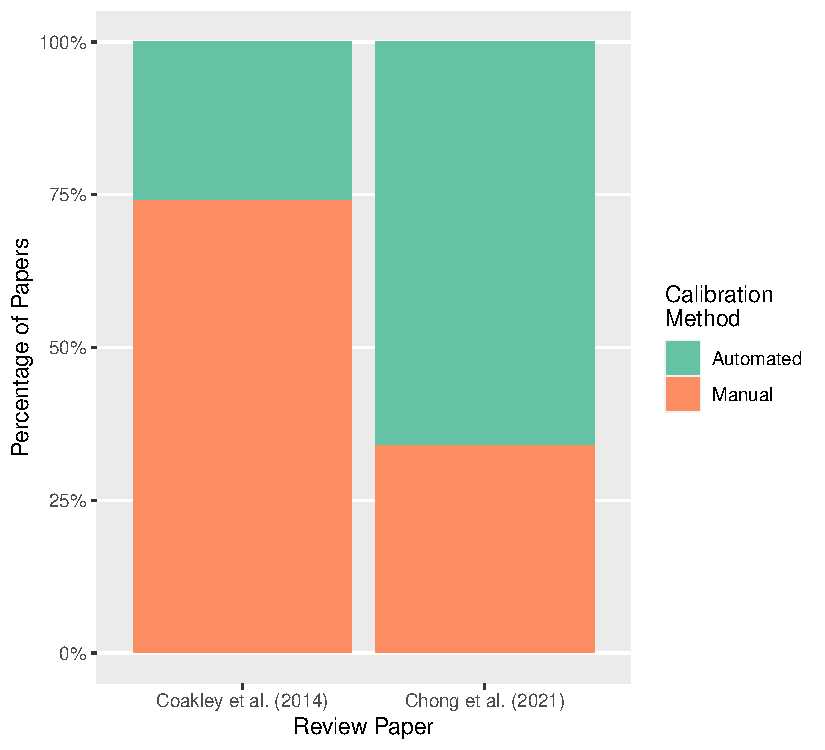
\includegraphics[width=\textwidth]{figures/auto_manual.pdf}
\caption{Type of calibration approach (Automated or Manual) (left pie-chart); and most commonly used methods for the automated calibration of building energy simulation models (right bar-plot).}
\label{fig:auto_manual}
\end{figure}

\begin{table*}[h!]
\caption{Applications, R packages, Python libraries and code repositories for performing sensitivity analysis, optimization, and Bayesian inference algorithms on building energy simulation models.} 
\label{tab:open_source}
\centering
\resizebox{\textwidth}{!}{\begin{tabular}{p{0.15\linewidth} p{0.2\linewidth} p{0.125\linewidth} p{0.425\linewidth} p{0.1\linewidth}}
  \hline
  \hline
  \textbf{Name} & \textbf{Type} & \textbf{Language} & \textbf{Method(s)} & \textbf{Ref.} \\
  \hline
  \hline
  \multicolumn{4}{l}{\underline{Sensitivity Analysis}}  \\
  sensitivity & CRAN & R & SRC, SRRC, PRCC, Morris, FAST, Sobol & \cite{sensitivity_r}\\
  SALib & PyPI/GitHub & Python & Morris, FAST, Sobol & \cite{herman2017salib}\\
  \multicolumn{4}{l}{\underline{Optimization-based calibration}}  \\
  GenOpt & Application & Java & GPSHJ, PSO  & \cite{wetter2001genopt}\\
  jEPlus & Application & Java & NSGA-II & \cite{jeplus}\\
  DEAP & PyPI/GitHub & Python & NSGA-II, PSO & \cite{fortin2012deap}\\
  ecr & CRAN/GitHub & R & NSGA-II, PSO & \cite{ecr_r}\\
  \multicolumn{4}{l}{\underline{Bayesian calibration}} \\
  SAVE & CRAN/GitHub & R & Bayesian emulation, calibration, and validation following Bayarri et al. \cite{bayarri2007framework} with roots in Kennedy and O'Hagan \cite{kennedy2001bayesian} and Higdon et al. \cite{higdon2004combining} & \cite{save_r}\\
  bc-stan & GitHub & R & Bayesian emulation and calibration following Kennedy and O'Hagan \cite{kennedy2001bayesian} and Higdon et al. \cite{higdon2004combining} & \cite{chong2018guidelines}\\
  pySIP & GitHub & Python & Bayesian emulation and calibration for continuous time stochastic state-space (e.g. RC networks) & \cite{raillon2019pysip}\\
  \hline
  \hline
\end{tabular}}
\raggedright \footnotesize Abbreviations: PyPI (Python Package Index); CRAN (Comprehensive R Archive Network); SRC (Standardized Regression Coefficients); PRCC (Partial Rank Correlation Coefficient); SRRC (Standardized Rank Regression Correlation); FAST (Fourier Amplitude Sensitivity Testing); GPSHJ (Generalized Pattern Search Hooke Jeeves); PSO (Particle Swarm Optimization); NSGA-II (Non-dominated sorting genetic algorithm II); 
\end{table*}

\subsubsection{Optimization-based calibration}

Genetic algorithm (GA) \cite{bandera2017towards, ramosruiz2017analysis, ramosruiz2016genetic, zuhaib2019application, martinez2020performance, martinez2020model, nagpal2019framework, tian2019investigation, chen2019meta}, particle swarm optimization (PSO) \cite{andrade-cabrera2017ensemble, yang2016automated, roberti2015calibrating, andrade-cabrera2019augmented, zhang2020development, Ha2020parameter, larochellemartin2019energy, ferrara2020optimizing, cacabelos2017development}, and the Hooke-Jeeves (HJ) algorithm \cite{li2018stepwise, abdelalim2017data, ogando2017energy, carlon2016on, cacabelos2017development} are the most widely used algorithms for optimization-based calibration. Both GA and PSO belong to the class of evolutionary algorithms that are population-based with a metaheuristic characteristic. GA is inspired by the process of natural selection and optimizes using biological operators such as mutation, crossover and selection. Specifically, the non-dominated sorting genetic algorithm II (NSGA-II) algorithm has been extensively applied for the optimization-based calibration of BES models \cite{bandera2017towards, ramosruiz2017analysis, ramosruiz2016genetic, zuhaib2019application, martinez2020performance, martinez2020model} because of its ability to obtain a better spread of solutions and convergence than other multi-objective evolutionary algorithms \cite{deb2002fast}. Proposed by Kennedy and Eberhart \cite{kennedy1995particle}, PSO optimizes via swarm intelligence and is inspired by the social behavior of organisms in groups such as a bird flock or a fish school. Lastly, the HJ algorithm \cite{hooke1961direct} belong to the family of generalized pattern search (GPS) algorithms and has gained popularity in BES because the number of function evaluations increases only linearly with the number of design parameters \cite{wetter2001genopt}.

A common feature of the GA, PSO, and HJ algorithm is that they are all gradient-free. Therefore, they are suitable for optimization frameworks that minimize a cost function that needs to be evaluated by an external BES program. Additionally, population-based metaheuristic algorithms such as PSO and GA initializes the optimization with a population of randomly distributed points to reduce the risk of converging to local minima. However, situations of falling far from the pareto-optimal front can be hard to detect, and therefore defining a stopping criteria is difficult. Although guidelines \cite{ashrae2014guideline, evo2012international, femp2015guidelines} specifying thresholds for accuracy metrics such as CV(RMSE) and NMBE are often used, it has been shown that these are not proper stopping criteria for automatic optimization-based calibration \cite{martinez2020performance}. Nonetheless, minimizing CV(RMSE) was also found to be the most robust cost function under different combinations of error metrics, calibration output, and calibration dataset time resolution \cite{martinez2020performance}. Constraints in the form of a specified range for the input parameters are often added to prevent unreasonable values \cite{qiu2018quick}.  

Optimization-based calibration has been widely applied in BES (Fig. \ref{fig:auto_manual}). A prominent example is the Autotune project that aims to replace manual calibration with a calibration method that leverages supercomputing, large databases of simulation results, and an evolutionary algorithm to automate the calibration process \cite{chaudhary2016evaluation, garrett2015scalable}. Sun et al. \cite{sun2016pattern} proposed a pattern-based optimization approach that determines the parameters to tune based on whether the identified bias is universal or seasonal \footnote{Universal bias occurs when the monthly utility bill is consistently higher or lower than the simulation predictions. In contrast, a seasonal bias is denoted by utility bills that are partially higher and lower than the simulation predictions.}. Yang and Becerik-Gerber \cite{yang2015model} performed independent single objective optimization at the component, zone, and building level. The union of the independent solution sets is then used for the subsequent multi-objective optimization. 

Optimization has also been used for the calibration of building components and sub-systems such as models of BIPV \cite{Ha2020parameter}, absorption thermal energy storage \cite{schreiber2018predicting}, and components of the air-handling unit \cite{larochellemartin2019energy}. Likewise, optimization has been used to calibrate UBEMs. Santos et al. \cite{santos2018evaluating} calibrated 56 buildings in a district using GA while considering the urban heat island effect. Zekar and Khatib \cite{zekar2018development} applied optimization for the calibration of an urban-scale RC model. Since numerical optimization can be computationally impractical at the urban-scale, optimization-based calibration of UBEMs often involves first parameter reduction in the form of day typing, zone typing, and the use of archetypes. 

\subsubsection{Calibration under uncertainty}

Uncertainty is an inevitable characteristic of BES models because of the complexity and interactions between different building systems. In many building energy applications, uncertainty management is an important aspect when accounting for risk in the decision-making process. It is somewhat surprising that only 32 of the 108 ($\sim$30\%) papers reviewed involved some form of uncertainty quantification during model calibration. 

\paragraph{Types and sources of uncertainty}

In general, uncertainty can be classified as either aleatory or epistemic \cite{tian2018review, roy2011comprehensive}. Aleatory uncertainty (or irreducible uncertainty) is the uncertainty caused by inherent variations or randomness of the building system or sub-system under investigation that cannot be explained by the data collected. In contrast, epistemic uncertainty (or reducible uncertainty) is the uncertainty that arises from a lack of knowledge (or data). The distinction between aleatory and epistemic uncertainty has merit in guiding the uncertainties that have the potential of being reduced \cite{der2009aleatory}. However, developing BES models involves a significant degree of subjectivity that depends on the data available that may also evolve throughout a building's lifecycle. As a result, most uncertainties are often a combination of both aleatory and epistemic uncertainty, making it difficult to distinguish between the two. 

Related to the types of uncertainty is the identification and classification of uncertainty by their sources, which forms an important part of a comprehensive uncertainty quantification framework \cite{roy2011comprehensive, sun2014closing}. In the context of BES calibration, there are two sources of uncertainty:
\begin{itemize}
    \item Parameter uncertainty: Uncertainty associated with influential model inputs that are not known with certainty. 
    \item Model form uncertainty: Model discrepancy (also called model inadequacy) that results from all assumptions, conceptualizations, abstractions, and approximations of the real-world physical processes. 
\end{itemize}

\paragraph{Uncertainty quantification}

Uncertainty quantification in BES can be broadly categorized as either forward or inverse. Forward approaches quantify uncertainty in the model output(s) by propagating them from uncertainties in the input parameters (Fig. \ref{fig:forward}). Statistical sampling techniques such as Monte Carlo simulation or Latin Hypercube Sampling are easy to apply and the most common in the field of BES \cite{yun2017development, harmer2015using, cipriano2015evaluation, sakiyama2020natural, giuliani2016modeling}.

\begin{figure}[!h]
\centering
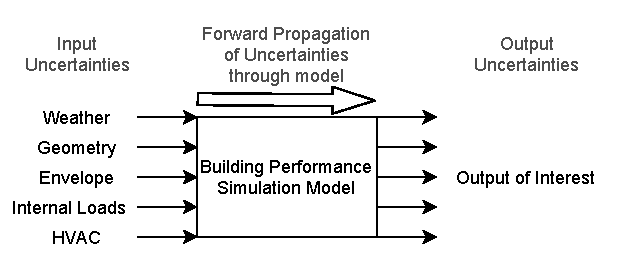
\includegraphics[width=0.8\textwidth]{figures/forward_uncertainty.pdf}
\caption{Forward approach to uncertainty quantification by propagating input uncertainties to obtain uncertainties in the output of interest.}
\label{fig:forward}
\end{figure}

Inverse approaches involve quantifying various sources of uncertainties given a set of observations from the building system being modeled. In particular, the calibration paradigm known as Bayesian calibration has gained popularity in BES due to its ability to naturally incorporate uncertainty and combine prior information (based on existing or expert knowledge) with measured data (through a likelihood function) to derive posterior estimates of the model parameters (Eq. \ref{eq:bayesTheorem}). As shown in Fig. \ref{fig:auto_manual} (above), Bayesian calibration was applied in about one-third of the studies that utilized an automated approach. 

\begin{equation}\label{eq:bayesTheorem}
p(t\mid y)\propto p(y \mid t) \times p(t)
\end{equation}

A notable approach within the Bayesian calibration paradigm is the formulation
proposed by Kennedy and O'Hagan (KOH) \cite{kennedy2001bayesian}. KOH's approach differs from traditional approaches by allowing for various sources of uncertainty and attempting to correct for any model inadequacy or bias (Eq. \ref{eq:koh}). There have been several applications of KOH's approach in the field of BES calibration \cite{martinez2019energy, menberg2019influence, chong2017bayesian, yuan2017simultaneous,li2016assessment, heo2015evaluation, chong2019continuous, chen2019district, tardioli2020methodology}, including a detailed guideline for its application in the field \cite{chong2018guidelines}. 

\begin{equation}\label{eq:koh}
y(x) = \eta(x,t) + \delta(x) + \epsilon(x)
\end{equation}

\noindent where, $y(x)$ is the observed field measurement, $\eta(x,t)$ is the output of the BES given observable inputs $x$ and calibration parameters $t$, $\delta(x)$ is the model inadequacy, and $\epsilon(x)$ is the observation errors. 

Other noteworthy approaches include Bayesian hierarchical modeling for the calibrating of urban-scale building energy models \cite{kristensen2018hierarchical, kristensen2020long} and sequential updating taking advantage of Bayes theorem to keep the model up to date without losing past knowledge \cite{chong2019continuous, rouchier2019sequential}.

Given the complexity of BES models, posterior distributions often cannot be derived analytically. Consequently, Markov chain Monte Carlo (MCMC) is often used in Bayesian calibration to sample from the posterior distributions because of its flexibility and straightforward application to complex problems. However, it is well known that performing Bayesian inference via MCMC is computationally expensive especially when likelihood evaluations involve computationally expensive models such as in the case of BES. 

To alleviate the high computation cost of Bayesian inference, metamodels have been proposed as surrogates of the energy model. Gaussian processes (GP) \cite{martinez2019energy, menberg2019influence, chong2018guidelines, lim2017comprehensive, chong2017bayesian, yuan2017simultaneous, kim2016stepwise, chong2019continuous, chen2019district} and linear regression \cite{lim2018influences, sokol2017validation, li2016assessment, tian2016identifying, tardioli2020methodology} are the most popular with competing trade-offs between computation cost and accuracy.  Additionally, more efficient MCMC sampling strategies such as Hamiltonian Monte Carlo (HMC) \cite{chong2017bayesian, lundstrom2019bayesian} and Approximate Bayesian Computation (ABC) methods that provide estimates of the posterior distributions without having to compute the likelihood function \cite{zhu2020uncertainty} have also been proposed to reduce computation cost. 

\subsection{Analytical Tools and Techniques} \label{sec:analytical_tools}

Analytical tools and techniques are often applied to both manual or automated calibration approaches. Following an extensive review of calibration methods, Coakley et al. \cite{coakley2014review} list these techniques with detailed explanations. Table \ref{tab:analytical} presents a subset of the techniques \cite{coakley2014review} that is relevant to this review. As can be seen from Table \ref{tab:analytical}, We do not extend the classifications proposed in \cite{coakley2014review} but augment their descriptions so that it encompasses the publications reviewed.

\begin{table*}[h!]
\caption{Analytical tools and techniques that were used to support the calibration process applied in the papers reviewed. Adapted from \cite{coakley2014review}.} 
\label{tab:analytical}
\centering
\resizebox{!}{0.4\textheight}{\begin{tabular}{p{0.15\linewidth} p{0.3\linewidth} p{0.85\linewidth}}
  \hline
  Acronym & Name & Description \\
  \hline
  SA & Sensitivity analysis &  Used to provide insights on how variations in uncertain inputs map onto the outputs. Can be used to identify non-influential parameters that are ignored during calibration or to help set priorities for future efforts (e.g. identify important parameters for measurements or detailed investigation). \\
  HIGH & High-res data & Utilizes data at hourly (or sub-hourly) resolutions as opposed to daily or monthly temporal resolution data \\
  AUDIT & Detailed audit & Conducting detailed audits to gain a better knowledge of the building systems or sub-systems. \\
  UQ & Uncertainty quantification & The assessment of parameter uncertainty as part of the calibration process. \\
  EXPERT & Expert knowledge / templates / model database & Approach which utilize expert knowledge or judgment as a key element of the process. Often involves the use of databases or templates of typical building parameters and components to reduce user input requirements.\\
  PARRED & Parameter reduction & Involves reducing the number of model input parameters. Examples include day-typing (reducing detailed schedules into typical day-type schedules), zone-typing (aggregating spaces with similar thermal zones) or building archetypes (grouping buildings into representative archetypes for urban-scale model calibration) \\
  BASE & Base-case modeling & The use of measured base-loads to calibrate the building model. Calibration is carried out during the base-case when (a) heating and cooling loads are minimal and the building is dominated by internal loads, thus minimizing the impact of weather-dependent variables, or (b) internal loads are minimal and the HVAC system is not operating to better characterize weather dependent variables such as the building envelope when internal temperatures are free-floating. \\  
  EVIDENCE & Evidence-based model development & Approaches that implement a procedural approach to model development, making changes according to source evidence rather than ad-hoc intervention. Often requires model development version controls to keep track of the changes. & \cite{raftery2011calibrating} \\
  SIG & Signature analysis & The use of graphical analysis techniques to identify the impacts of different input parameters on the model output of interest. \\
  STEM & Short-term energy monitoring & On-site measurements for a short period of time. Typically used to identify typical energy end-use profiles and/or base-loads. \\
  INT & Intrusive testing & Intrusive techniques involving interventions in the operation of the actual building. \\
  \hline
\end{tabular}}
\end{table*}

Fig. \ref{fig:analytical} provides an overview of the number of papers employing a certain analytical technique to assist or complete the calibration process. What stands out in the figure is that the application of sensitivity analysis (SA) and the use of high-resolution data have the highest frequency. SA is closely connected with model calibration because it can be used to provide insights on how variations in uncertain parameters affect variations in calibration performance \cite{pianosi2016sensitivity}. Likewise, the use of high-resolution data is not surprising with the proliferation of IoT devices and sensor networks in buildings making hourly and sub-metered data more readily available for calibration. 

\begin{figure}[!h]
\centering
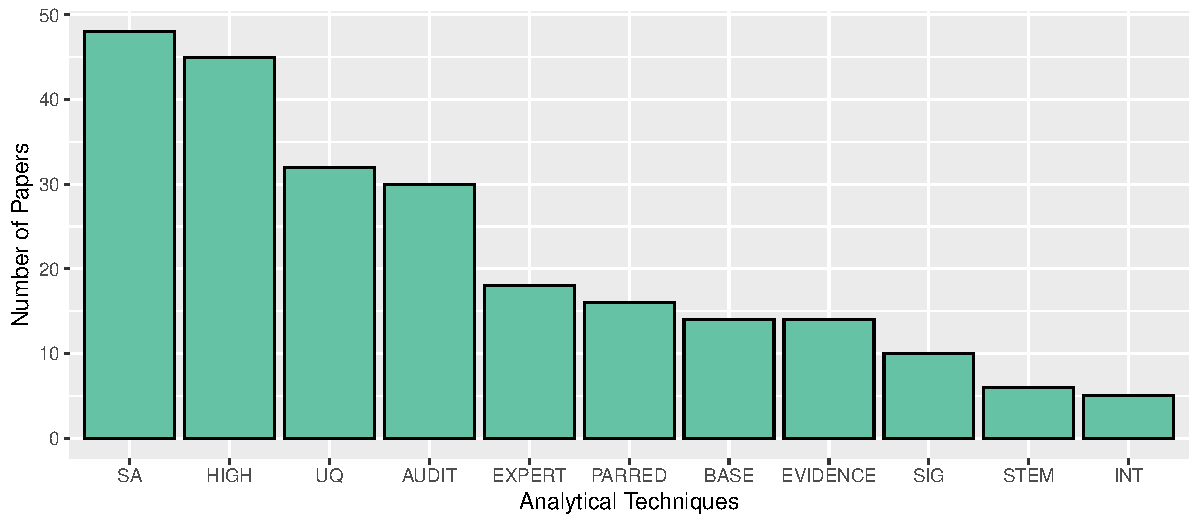
\includegraphics[width=\textwidth]{figures/analytical.pdf}
\caption{Analytical techniques used in the papers reviewed for both manual and automated calibration approaches. Calibration processes can involve more than one analytical technique. Therefore, the values do not add up to the total number of papers reviewed (N=107).}
\label{fig:analytical}
\end{figure}

\subsubsection{Sensitivity Analysis}

The results of this review confirm the close association between sensitivity analysis (SA) and model calibration, especially among automated calibration processes. Evidence from this review shows that the most commonly applied SA methods in BES are screening methods followed by perturbation, regression, variance, metamodel, and regional sensitivity analysis (RSA) methods (Fig. \ref{fig:sa}). Screening, regression, variance, metamodel, and RSA methods are global SA methods that consider output variability over the entire range of input variations while perturbation is a local SA method that considers output variability based on input variations around a specified base value. 

\begin{figure}[h!]
\centering
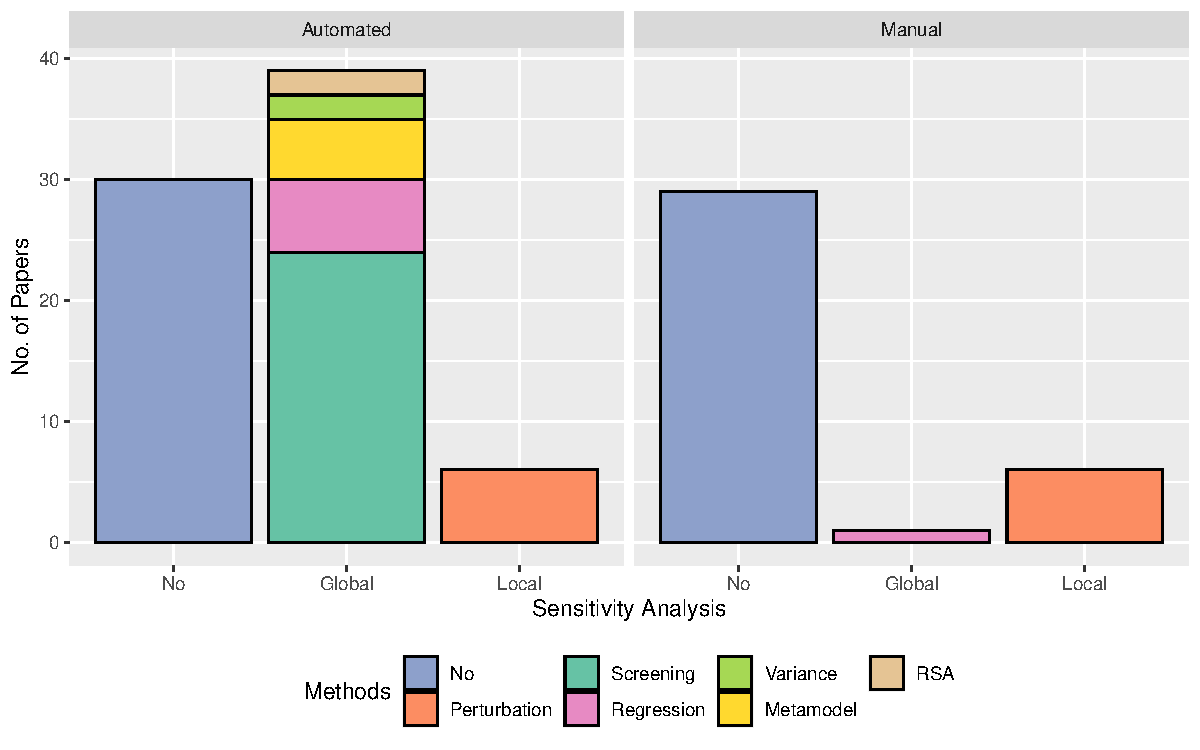
\includegraphics[width=0.6\textwidth]{figures/sa.pdf}
\caption{Types of sensitivity analysis used in building energy simulation.}
\label{fig:sa}
\end{figure}

In this review, variance-based SA methods are not common because they are computationally demanding requiring large sample sizes for accurate approximations of the sensitivity indices. Suppose that there are $t$ uncertain parameters, the approximate number of model evaluations required is approximately $t$ for perturbation local SA methods; $10-100 t$ for screening methods; $100-1000 t$ for regression and RSA methods; and $>1000t$ for variance-based methods \cite{pianosi2016sensitivity}. Consequently, Metamodels, surrogates or emulators are typically used in place of computationally expensive simulation runs required by computationally demanding SA methods \cite{pianosi2016sensitivity}. In BES, this is a two-stage process that involves the creation of a metamodel followed by the calculation of sensitivity measures using the meta-model based on the variance-based SA method \cite{tian2013review}. Specific choices of metamodels may also provide sensitivity measures that can be used to rank input parameters according to their influence on the output of interest. Examples include the use of random forest variable importance \cite{tian2016identifying, lim2017comprehensive, lim2018influences} and estimates of marginal posterior using Gaussian processes \cite{yuan2017simultaneous}.

Screening methods are popular due to their low computation cost compared to other global SA methods, making it suitable for BES models that are typically non-linear with high-dimensional parameter space. The method of Morris \cite{morris1991factorial} is the most established and widely used screening method. Sampling for the Morris method is carried out by randomly selecting $r$ starting points that are perturbed One-at-A-Time (OAT). The computation cost is therefore $r(t+1)$ for $t$ input parameters. A measure of global sensitivity is commonly obtained using the $r$ trajectories to compute the mean $\mu$ \cite{morris1991factorial} or the modified mean $\mu^*$ proposed by \cite{campolongo2007effective}. In general, most studies rely on graphical plots of $\mu$ (or $\mu^*$) and $\sigma$ for better interpretability when screening out non-influential parameters \cite{martinez2019energy, kristensen2018hierarchical, chong2017bayesian, chong2018guidelines, chong2019continuous,li2018stepwise, kim2016development, ramosruiz2016genetic, yang2015model, zuhaib2019application, larochellemartin2019energy, martinez2020model, ferrara2020optimizing}. Others consider only $\mu$ (or $\mu^*$) and use it to rank and identify dominant parameters \cite{heo2015evaluation, chen2019district, wang2020bayesian, zhang2020development, giuliani2016modeling, roberti2015calibrating}.

Perturbation methods are the simplest type of SA and involve varying (perturbing) the model inputs from their base or nominal values One-At-a-Time (OAT). Compared with global SA methods, the advantages of perturbation methods include (1) its ease of application and interpretation \cite{tian2013review}, and (2) requiring the least number of model evaluations \cite{pianosi2016sensitivity}. The order of influence is often used to identify a subset of parameters to be calibrated \cite{robertson2015reduced, sun2016pattern, enriquez2017towards, tuysuz2020calibrating, kim2015development, kim2016development, elharidi2017energy, glasgo2017assessing}. Sun et al. \cite{sun2016pattern} illustrate this clearly by using parametric perturbation to identify a priority list of 17 calibration parameters that would be adjusted within a pattern-based automated calibration framework. On the other hand, studies have also applied perturbation methods after the calibration to investigate possible causes for remaining discrepancies between simulated and measured data \cite{allard2018energy} or to determine if the calibrated model is robust to uncertainties in particular input factors \cite{mihai2017bottom}. 

Regression methods refer to the use of regression or correlation coefficients to derive information about output sensitivity to variations in input uncertainty. The input/output dataset is often generated using Monte Carlo simulation or Latin Hypercube Sampling. Several types of regression or correlation coefficients have been used as sensitivity measures in building energy analysis  \cite{tian2013review}. The choice depends on linearity and monotonicity assumptions between the inputs and output \cite{pianosi2016sensitivity}. In this review, we found that Standardized Regression Coefficients (SRC) was most commonly applied \cite{lim2018influences, qiu2018quick, lim2017comprehensive, tian2016identifying} with some studies employing partial rank correlation coefficient (PRCC) \cite{andrade-cabrera2019augmented} and standardized rank regression correlation (SRCC) \cite{ascione2020real}. The advantage of regression-based approaches lies in their ease and simplicity in application. 

\subsubsection{Analytical techniques by approach and application}

Fig. \ref{fig:analytical_approach} shows the breakdown of analytical techniques according to the calibration approach (manual or automated) and the spatial scale (component/system, building, or urban). The results, as shown in Fig. \ref{fig:analytical_approach} indicates that sensitivity analysis (SA), high-resolution data, uncertainty quantification (UQ), and building audits are the most commonly applied in automated approaches. Comparatively, SA is not as widely used in manual calibration approaches. 20\% of the papers utilizing manual approaches involve applying SA in contrast with 65\% of the papers for automated approaches. A possible explanation is that equfinality issues are especially challenging for automated approaches since objective functions are normally designed to minimize discrepancies between simulated and observed responses. This might produce a model with a higher prediction accuracy, but it might not inform the modeler about the true parameter values \cite{beven2006manifesto}. In contrast, manual approaches adjust the calibration parameters based on heuristics that are based on the expertise of an experienced modeler. Therefore, issues of identifiability are not as critical in manual approaches. 

\begin{figure}[!h]
\centering
\includegraphics[width=\textwidth]{figures/analytical_approach_scale.pdf}
\caption{Analytical techniques used in the papers reviewed grouped by the corresponding spatial scale (left plot) and calibration approach (right plot). Calibration processes can involve more than one analytical technique. Therefore, the values do not add up to the total number of papers reviewed (N=107).}
\label{fig:analytical_approach}
\end{figure}

Moving on to model calibration at different spatial scales, it can be observed that SA, high-resolution data, UQ, and building audits are prevalent at the building-scale. On the contrary, parameter reduction and expert knowledge are the predominant analytical techniques for urban scale model calibration efforts. Parameter reduction aims to reduce the number of model inputs by characterizing and grouping similar inputs to reduce the complexity of the model while preserving the final decision based on the full set of parameters. Well-known examples of parameter reduction techniques in BES are day-typing (grouping schedules with similar profile) and zone-typing (grouping similar thermal zones) \cite{coakley2014review}. At the urban-scale, archetypes are commonly used to reduce the number of model inputs and therefore the effort and cost of modeling distinct buildings \cite{sokol2017validation, fernandez2020novel, kristensen2020long, tardioli2020methodology, hedegaard2019bottom, wang2020bayesian, chen2020automatic}. 

Archetype generation involves two steps, segmentation followed by characterization \cite{reinhart2016urban}. Segmentation divides buildings with similar characteristics based on key parameters such as building type, construction year or period, floor area, building height, and/or shape (if geometry data is not available) \cite{sokol2017validation, fernandez2020novel, kristensen2020long, tardioli2020methodology}. What follows is the characterization of building construction and operation properties based on expert knowledge that involves deriving input values from existing databases, building codes and standards, and representations of national building typologies (also referred to as reference buildings). For example, several studies \cite{kristensen2020long, hedegaard2019bottom, wang2020bayesian} modeled construction properties (inferred from construction year) using information from the TABULA (2009-2012) and EPISCOPE (2013-2016) projects \cite{ballarini2014use,loga2016tabula} that were aimed at providing national residential building typologies for various European countries. Another example is the use of the U.S. Commercial Buildings Energy Consumption Survey (CBECS) and the U.S. Residential Energy Consumption Survey (RECS) databases to derive detailed information on the construction and operation of the buildings (e.g. insulation levels, internal loads and schedules, mechanical systems, and hot water consumption) \cite{taylor2019multi, sokol2017validation}. Likewise, Chen, Deng and Hong \cite{chen2020automatic} derived input values based on the minimum energy efficiency requirements in the California's building energy efficiency standards Title 24 while Krayem et al. \cite{krayem2019urban} defined internal loads and schedules following the ASHRAE 90.1 Standard.

\subsection{Multi-stage calibration} \label{sec:multi-stage}

Supporting multi-stage calibration through a combination of data from building information models (BIM), as-built documents, on-site audits, occupancy sensors, indoor environmental quality (IEQ) sensors, the building management system (BMS), and metered HVAC component energy consumption may not be a far-fetched reality that is only possible for state-of-the-art buildings as building data becomes more easily available and accessible.

Multi-stage calibration is of interest because it is often proposed to more accurately represent the building being modeled. Since calibration is an under-determined problem \cite{chong2018guidelines}, it is possible for a model that is calibrated at a coarser spatial or temporal level to meet the most stringent error thresholds without accurately representing the building at finer spatial or temporal levels \cite{zuhaib2019application, yin2016linking, raftery2011calibrating}. It has been argued that it is crucial to achieve simultaneous accuracy at multiple levels of the simulation to correctly provide insights at the respective levels. For instance, Yang and Becerik-Gerber \cite{yang2015model} asserts that building level accuracy is needed to provide insights on overall energy performance but an ECM level accuracy would be needed for estimating the energy savings potential of different ECMs. Similarly, Li et al. \cite{li2015why} showed using statistical hypothesis testing that an energy model calibrated for one ECM cannot be used to accurately cross-estimate the energy consumption of another ECM. 

Our review found that calibrating the model with data of the building under free-floating conditions is a dominant feature of multi-stage approaches \cite{cipriano2015evaluation, aparicio-fernandez2019energy, cacabelos2017development, ferrara2020optimizing}. Such a base-case method is often employed because the number of uncertain parameters is substantial reduced when there are little or no internal loads (in particular occupancy) and the HVAC system is not operating. Additionally, it is well-known that occupancy is a highly uncertain model input \cite{yan2015occupant} with significant influence on the predictive accuracy of a calibrated energy model \cite{li2015why, kim2017building, chong2021occupancy}. Consequently, parameters like envelope material thermal properties and infiltration rates are more straightforward to identify during periods when the building is free-floating (Fig. \ref{fig:target_param} in Section \ref{sec:output_param}). 


\section{Discussion}

\subsection{Credibility or predictive accuracy} \label{sec:credibility}

It is apparent from this review that predictive accuracy is widely used to evaluate BES models. However, a model with low predictive accuracy might still be reasonable for its intended use. For example, a comparative analysis rather than absolute predictive accuracy would suffice when deciding between different retrofit scenarios. Likewise, it is also possible for a BES model to exhibit a good fit to observation data but not accurately represent building systems or sub-systems due to many input parameters and uncertainties. Chong and Menberg \cite{chong2018guidelines} demonstrated that a low CV(RMSE) and NMBE is not indicative of good estimates of the true values of the calibration parameters. 

The Cambridge English dictionary defines credibility as ``can be believed or trusted''. From a modeling standpoint, credibility would not require the model to be accurate or have high fidelity. For example, Yin, Kiliccote, and Piette \cite{yin2016linking} evaluated an EnergyPlus model's prediction of dynamic response by field-testing a set of demand response control strategies. As pointed by Rykiel \cite{rykiel1996testing}, the crux of the issue is therefore determining (1) if a model is acceptable for its intended purpose; and (2) how confident should we be about the model's inference about the actual building system. Similar concepts of fit-for-purpose modeling strategies were also discussed in BES, emphasizing the need to consider the aim of the simulation when selecting different modeling approaches \cite{trvcka2010overview, gaetani2016occupant, gaetani2020stepwise, chong2021occupancy, zhan2021data}. 

Likewise, the choice of model and calibration approach should not be decoupled from the intended purpose of the simulation. Simple models are more transparent, require less data for parameter estimation and calibration, and less prone to error propagation. Consequently, it is imperative that the purpose of the simulation and their corresponding performance criteria be specified before any calibration is carried out. However, current calibration studies rely solely on measures of accuracy such as CV(RMSE) and NMBE to determine whether a model is ``calibrated''. There is currently no guidance on how the credibility of BES models for various applications can be qualified. The association between model complexity, simulation objectives, and data informativeness is also poorly understood. Further research on this topic is therefore recommended. 

\subsection{Calibrating urban-scale models}

The result of this review indicates that approximately 15\% of the papers are at the urban-scale. Of the 15\%, most are located in the U.S. (54\%) and Europe (34\%), with none in a tropical climate. Since the urban context (inter-building effects and urban microclimate) is an important aspect that should be considered in UBEMs \cite{hong2020ten, miller2018urban}, it would be interesting to evaluate the performance of the UBEM calibration methodologies in the tropics and cities outside of the U.S. and Europe. 

This review also found that UBEMs are typically calibrated using monthly or annual data (Fig. \ref{fig:spatial_temporal}) and rely on expert knowledge and parameter reduction techniques (Fig. \ref{fig:analytical_approach}). This finding is consistent with previous studies, which found that the UBEM generation process typically relies on assumptions due to a lack of data quality and accessibility \cite{chen2019development, reinhart2016urban}. Consequently, the credibility of UBEMs is often questionable due to the widespread use of default or reference values, and the fact that UBEM calibration remains a significantly overparameterized problem. However, as discussed in the preceding section \ref{sec:credibility}, predictive accuracy is not synonymous to model credibility. The need for parsimonious models was also recently asserted in a review of UBEM use cases \cite{ang2020concept}.

With IoT and the proliferation of sensors in the built environment, wide-ranging data streams at increasing spatial and temporal scales may be more easily accessible in the future. Having access to large amounts of data entails other challenges such as ensuring data quality and consistency \cite{noardo2020tools, chen2019development}, and selecting only the necessary information needed for energy modeling \cite{biljecki2021extending}. However, it also brings the opportunity for future research that investigates the minimum level of complexity and data required to achieve a UBEM that is commensurate with its intended purpose. Data convergence across multiple spatial and temporal scales is needed to support such work. Additionally, an interdisciplinary team of modelers, urban planners, policymakers, and decision-makers more generally is necessary to address these challenges.

\subsection{Reproducible research in BES} \label{sec:reproduce}

In this review, we found that BES simulations and existing calibration approaches are difficult to reproduce from the publications alone because of the complexity of BES models, and the absence of clarity concerning the reporting of (a) calibration parameters, observed inputs, and observed outputs and (b) assumptions made during data pre- and post-processing.

BES models and the associated code and data should be made openly available to improve the quality of scientific research, reduce duplicated efforts, and facilitate collaborations \cite{pfenninger2017importance}. Furthermore, reproducibility will become increasingly difficult with increasing data sources and more complex calibration methodologies as we attempt to bridge the gap between simulation and reality. Without access to the code and the data, it would be almost impossible to implement the fundamentals of scientific research that includes transparency, rigor, and independent verification \cite{mcnutt2014journals, pfenninger2017importance}. 

While full reproducibility requires complete openness and familiarity with open-source toolkits, it is still valuable to open parts of the code and/or data. Therefore, we recommend an incremental approach to encourage reproducible research in BES. For a start, publications should include a checklist to ensure clear reporting of the context and processes involved in the calibration (Table \ref{tab:reproduce}). Next, all code should be published. The code only needs to be available and does not need to be structured or clean. Even poorly written code informs a lot about the calibration approach. Additionally, a subset of the data or synthetic data can be used where data privacy is of concern. 

\begin{table*}[h!]
\caption{Checklist for improving reproducibility of publications that involves the calibration of building energy simulation models.} 
\label{tab:reproduce}
\centering
\resizebox{\textwidth}{!}{\begin{tabular}{l }
  \hline
  \textbf{Checklist to enhance reproducibility}  \\
  \hline
  \underline{General Information} \\
  Aim of the simulation \\
  Building location (Longitude and Latitude) \\
  Building typology \\
  Weatherfile \\
  Total, conditioned and unconditioned floor area \\
  Simulation engine \\
  \underline{Measured Data} \\
  Observed output(s) and data source\\
  Observed input(s) and data source \\
  Pre-processing \\
  \underline{Calibration Method} \\
  Calibration parameters and their corresponding ranges\\
  Calibration approach (Automated or Manual) and algorithm if an automated approach was used\\
  Analytical tools and techniques (see section \ref{sec:analytical_tools}) \\
  Calibration sequence if a multi-stage sequential approach is involved \\
  \underline{Results and Conclusion} \\
  Post-processing \\
  Recommendation \\
  \hline
\end{tabular}}
\end{table*}

The technical challenges impeding reproducible publications can be summarized as poor documentation of the dependencies necessary for the code to run, imprecise documentation on how to install and run the associated code, and a lack of a robust way to run exact versions of all software involved \cite{boettiger2015introduction}. Additionally, the choice of either a permissive or copyleft license (i.e., legal terms) should be considered  \cite{pfenninger2018opening}. Docker is a popular platform that can provide the infrastructure to facilitate reproducible research in BES \cite{ball2020open, jia2021eplusr}. Specifically, Docker images and Dockerfiles are Docker concepts that help resolve the technical challenges to reproducibility mentioned at the start of this paragraph \cite{boettiger2015introduction}. To facilitate reproducibility, we created a GitHub repository (section \ref{sec:open}) to demonstrate a Docker based approach for reproducing BES research. 


\section{Conclusion}

There is currently no consensus in the BES community on the calibration procedures such as model inputs and outputs, calibration methods, calibration performance evaluation, and best practices to facilitate reproducibility. As a result, BES calibration has remained highly subjective and perhaps even elusive, and almost impossible to reproduce. Therefore, this study contributes to existing knowledge of BES calibration by providing a coherent and detailed summary of the data requirements and the current state of knowledge. Over a hundred journal articles from the past six years were synthesized and categorized based on each study's model inputs and outputs, location, data resolution, calibration method, and performance evaluation approach. 

The results indicate a lack of reproducibility due to the absence of clarity in reporting the modeling and data assumptions, calibration parameters, observed inputs, and observed outputs. Therefore, an incremental approach to encourage reproducibility in BES research was proposed in this study, along with a fully reproducible example on GitHub (section \ref{sec:open}). The more obvious finding to emerge from this review is that predictive accuracy is typically assumed to be synonymous with model credibility without stating the purpose of the simulation. The present study lays the groundwork that future calibration studies can build on. While it is clear that there is a significant body of work available, a culture of reproducibility will significantly aid efforts in establishing a standardized calibration methodology. 

\section*{Data availability} \label{sec:open}

The research compendium for this article can be found at \url{https://github.com/ideas-lab-nus/calibrating-building-simulation-review}, hosted at GitHub.

The simple example of reproducible building energy simulation (section \ref{sec:reproduce}) can be found at \url{https://github.com/ideas-lab-nus/reproducing-building-simulation}, hosted at GitHub.


%TC:ignore
\section*{CRediT authorship contribution statement}
\textbf{Adrian Chong:} Conceptualization, Methodology, Formal analysis, Investigation, Writing – Original Draft, Visualization, Supervision, Project administration. \textbf{Yaonan Gu:} Investigation, Data curation. \textbf{Hongyuan Jia:} Software, Data curation.


\section*{Acknowledgements}
This research is supported by the National University of Singapore, Singapore under its start-up grant (Project No. R-296-000-190-133).
%TC:endignore


\bibliography{scopus}

\end{document}